%--------------------
% Packages
% -------------------
\documentclass[11pt,a4paper,titlepage]{article}
\usepackage[utf8x]{inputenc}
\usepackage[T1]{fontenc}
%\usepackage{gentium}
\usepackage{mathptmx} % Use Times Font
\usepackage{amsmath}


\usepackage[pdftex]{graphicx} % Required for including pictures
\usepackage[english]{babel} % Swedish translations
\usepackage[pdftex,linkcolor=black,pdfborder={0 0 0}]{hyperref} % Format links for pdf
\usepackage{calc} % To reset the counter in the document after title page
\usepackage{enumitem} % Includes lists

\frenchspacing % No double spacing between sentences
\linespread{1.2} % Set linespace
\usepackage[a4paper, lmargin=0.1666\paperwidth, rmargin=0.1666\paperwidth, tmargin=0.1111\paperheight, bmargin=0.1111\paperheight]{geometry} %margins
%\usepackage{parskip}

\usepackage[all]{nowidow} % Tries to remove widows
\usepackage[protrusion=true,expansion=true]{microtype} % Improves typography, load after fontpackage is selected

%-----------------------
% Set pdf information and add title, fill in the fields
%-----------------------
\hypersetup{ 	
pdfsubject = {},
pdftitle = {},
pdfauthor = {}
}

%-----------------------
% Begin document
%-----------------------

\begin{document} %All text i dokumentet hamnar mellan dessa taggar, allt ovanför är formatering av dokumentet
\bibliographystyle{ieeetr}

\begin{titlepage}
  \centering
  \vspace*{2cm}
  {\Huge \textbf{\underline{CS-E4840}}}\\[0.5cm]
  {\Huge \textbf{\underline{\parbox{0.8\linewidth}{\centering Information Visualization D}}}}\\[1.0cm]
  {\Large \textbf{Assignment 3: Human Factors}} \\
  [1.0cm]
  {\Large Aleksi Kääriäinen (728971)}\\[1.0cm]
  {\Large \today}
\end{titlepage}

\section*{Introduction}
In this assignment, I have completed two visualization tasks using data relating to the SDG selected in assignment 1. Restating just for clarity, I picked SDG number 1, No poverty, for the topic of the assignments. Both tasks in this use the same dataset, that has also been used in assignments 1 and 2. The dataset includes data for the share of population living under the poverty line (daily income of US\$30) for most of the countries in the world in the time interval of years 1981-2019. The dataset is publicly available at \cite{data}.

\section{Maps and Colormaps}

In this task, I created two chorophleth maps using the poverty data. The graphs were created using \texttt{plotly}'s \texttt{choropleth} tool. Figure \ref{fig:viz1} shows the data colored with a sequential colormap, whereas figure \ref{fig:viz2} plots the data using a diverging colormap.

Figure \ref{fig:viz1} shows the share of population living under the poverty line for each country in 2015. The dataset used did not have data for every country in the world, missing countries are marked with grey on the map. Missing countries include Greenland, New Zealand, Libya etc. In the visualization, the darker the color, the larger the share of poverty in the country. The visualization shows clearly, that most of the countries in the world are poverty ridden even in the year 2015. I decided to use a yellow-red colormap, since humans usually associate a dark red color with something bad, and lighter colors with something more desirable.

\begin{figure}[h]
    \centering
    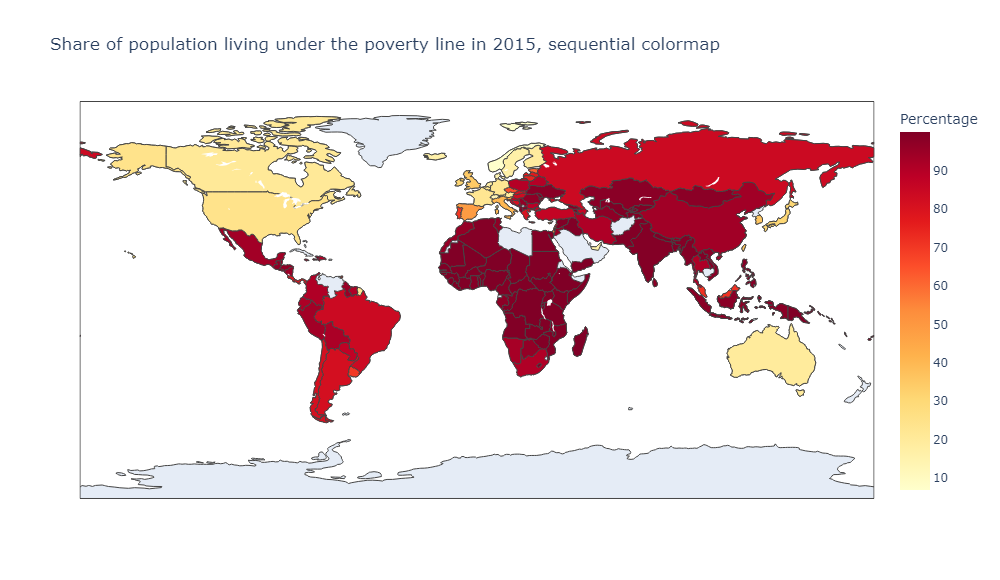
\includegraphics[width=1.0\linewidth]{reports/assignment-3/imgs/task1-1.png}
    \caption{Task 1 visualization (a)}
    \label{fig:viz1}
\end{figure}

The data used in figure \ref{fig:viz2} was shifted so that the neutral value was at 50\% with the formula:
\begin{align*}
x^{\prime} = x - 50,
\end{align*}
where $x$ is a vector of real numbers. Thus figure \ref{fig:viz2} showcases the countries' deviation from the 50\% share of population living in poverty. I used a blue-red colormap, where blue is in the negative values, and red in the positive values, creating a 'temperature' scale. It is in my opinion an intuitive way of visualizing a diverging dataset, since the connection to thermometers is so evident.

\begin{figure}[h]
    \centering
    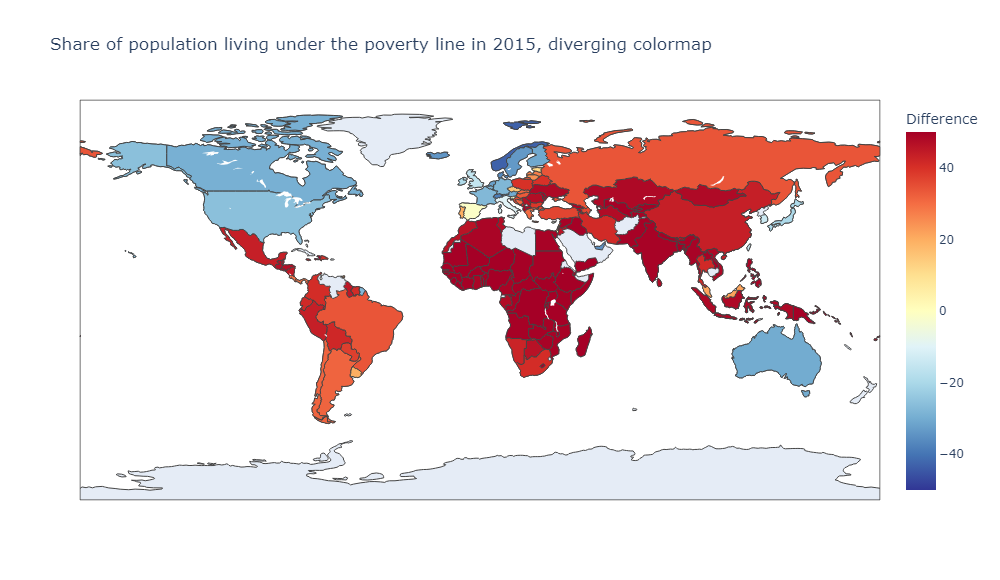
\includegraphics[width=1.0\linewidth]{reports/assignment-3/imgs/task1-2.png}
    \caption{Task 1 visualization (b)}
    \label{fig:viz2}
\end{figure}

I had no major challenges plotting the maps after finding the \texttt{plotly} library, which provides the ready made implementation for plotting choropleth maps. Reading the documentation of the functions helped to understand the different parameters needed and complete the task.

\section{Heatmaps and Clustermaps}

In this task, I visualized part of the dataset as a heatmap and a clustermap. In order to make the plots less cluttered, I used only a subset of the countries present in the dataset. I decided to visualize the evolution of the poverty rate in Central and Western European countries in the years 1981-2019. I used only those countries which have data for the full time interval, meaning that a few countries classified as Western or Central European are missing. There are 13 countries and 39 years in total, resulting in a 13x39 matrix used in the heatmaps.

\begin{figure}[h]
    \centering
    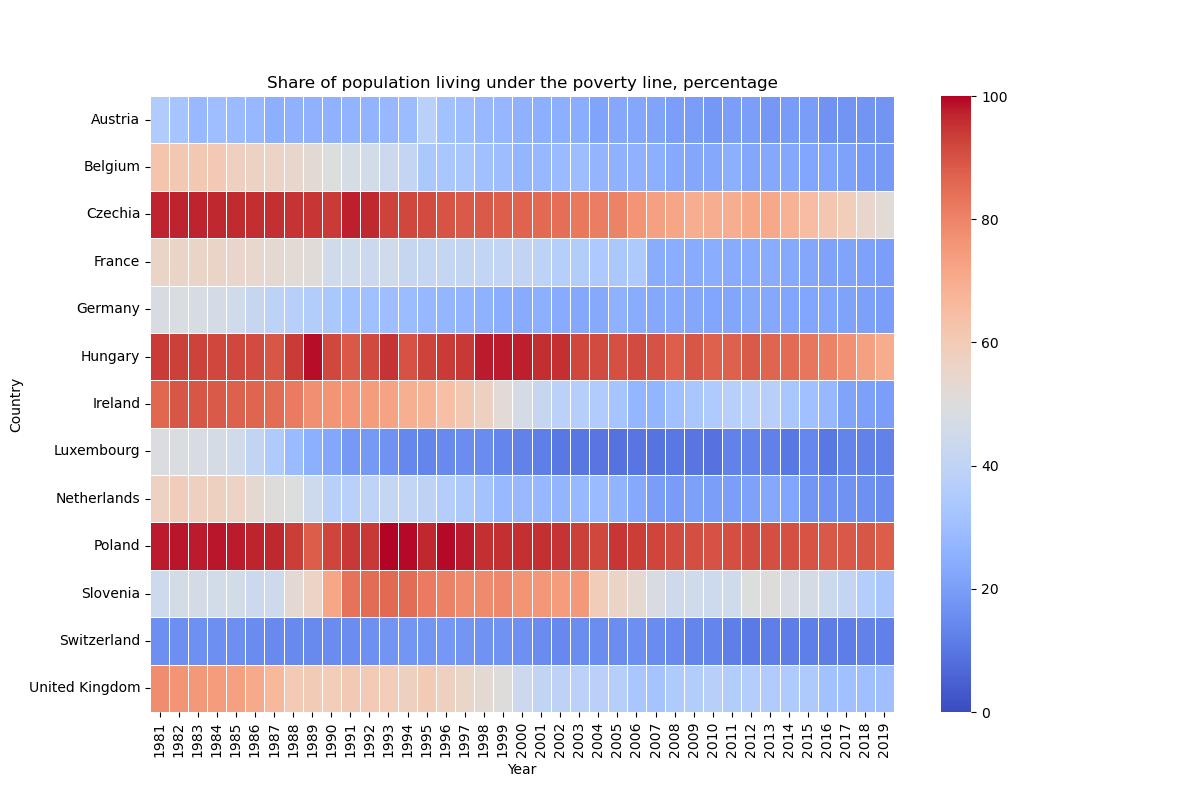
\includegraphics[width=1.0\linewidth]{reports/assignment-3/imgs/task2-1.png}
    \caption{Task 2 visualization (a)}
    \label{fig:viz3}
\end{figure}

Figure \ref{fig:viz3} shows the matrix plotted as a heatmap. The rows are countries in alphabetical order, and the years are also ordered. The colormap used is a diverging one, sliding from red to blue. The neutral value in this plot is 50. A diverging colormap shows instantly which values are below/above the neutral value and shows the differences between countries in a striking fashion. In my opinion, sorting the countries in alphabetical order does not ease reading the visualization much, but it does help fetching data for a single country. Maybe the benefits of alphabetical ordering would be more apparent, if more countries were used in the visualization.

\newpage

\begin{figure}[h!]
    \centering
    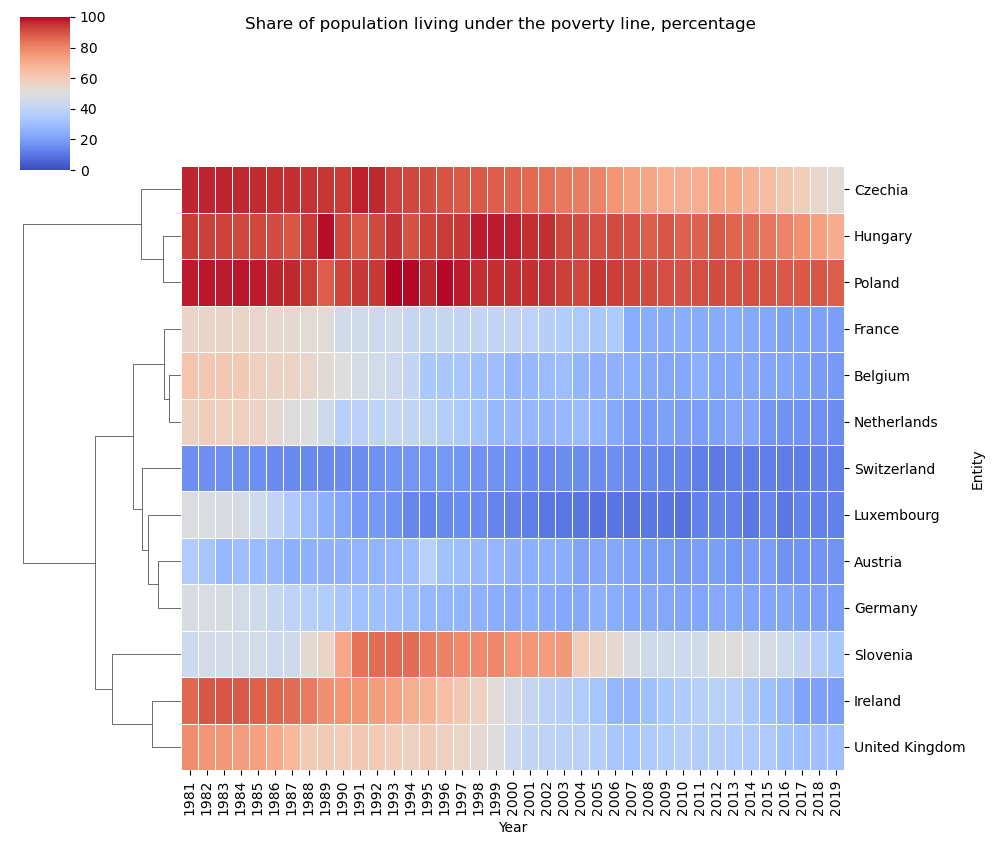
\includegraphics[width=1.0\linewidth]{reports/assignment-3/imgs/task2-2.png}
    \caption{Task 2 visualization (b)}
    \label{fig:viz4}
\end{figure}

Figure \ref{fig:viz4} shows the same data as in figure \ref{fig:viz3} this time plotted as a clustermap. The plot uses the same colormap for the same reasons as above. Clustering is done only on rows, since clustering the columns would have broken the temporal structure of the data. The similarity metric used for clustering is Euclidean distance, which is well suited for vectors of real numbers, and the clustering method is the average of clusters. Clustering by the average of the clusters works really well, as seen in the plot.

In my opinion, the clustermap is much easier to read since the rows have been clustered based on relative similarity, rather than sorted alphabetically. The clustering makes fetching answers to questions such as "Which countries have gotten wealthier over the years?" or "Which countries' share of poverty has stayed similar?" simple and quick.

I used the \texttt{seaborn} library for both visualizations in the task. At this point, \texttt{seaborn} is becoming pretty familiar to me. At first I had some trouble plotting the clustermap though. My code threw a cryptic error, but after studying the error and my data for a while, it turned out that the error was caused by NaN values in the data. After filtering out the rows that contained NaN values, the issue was fixed and I could complete the visualizations.

\newpage

\bibliography{reports/assignment-3/refs}

\end{document}